% !TEX root = Skin_Lesion_Classification_Using_Machine_Learning.tex

\section{Skin Lesion Classification Using Support Vector Machine [TN]}\label{sec:svm}
In this section we present a skin lesion classification approach by using Support Vector Machine (SVM). Therefor we first extract features out of the images that are then used as input data. Afterwards based on the extracted features we train and evaluate a SVM by making use of the Sklearn library \cite{scikit-learn}.   
\subsection{Feature Extraction [SPS]}

Feature extraction is the process of extracting relevant features that give information about the color,shape,texture etc. of the skin lesion.For extracting the features from the skin lesion it is mandatory to segment the skin lesion from the image and  then extract the features of the segmented lesion.In order to segment the lesion from the image , three segmentation techniques has been implemented.Initially an elliptical mask is applied to the image, and the skin lesion is extracted using the elliptical mask.Then features are extracted for the masked image and prepared as a data set.In the second segmentation technique which works on algorithm termed as watershed algorithm, the skin lesion is segmented based on peaks and valleys that are created based on the intensity gradient across the image.This kind of segmentation technique works really well on the images with no hair.But the images with hair , this type of segmentation did not work properly with hair as shown in the figure below.So after this segmentation technique the features are extracted and second data set is created.The final type of segmentation is done using k means clustering.It forms segmented regions using k clusters.The features for this kind of segmentation are extracted and then third data set is created.Based on the classification results from SVM, K means clustering technique found to give a better evaluation parameters like the high accuracy and high sensitivity.The features that were extracted after segmentation are listed as Moments, Huemoments,PCA features,Mean and Standard deviation of the color channels in the images,haralick features.
\subsubsection{Moments and Hu moments}
Image moments are a weighted average of image pixel intensities. Image moments capture information about the shape of a lesion in a binary image because they contain information about the intensity I(x,y) as well as position x and y of the pixels.The central moments are translation invariant. In other words, no matter where the lesion is in the image, if the shape is the same, the moments will be the same.       Hu Moments ( or rather Hu moment invariants ) are a set of 7 numbers calculated using central moments that are invariant to image transformations. The first 6 moments have been proved to be invariant to translation, scale, and rotation, and reflection. While the 7th moment’s sign changes for image reflection.
\subsubsection{Haralick features}
The basis for these features is the gray-level co-occurrence matrix . This matrix is square with dimension , where Ng is the number of gray levels in the image. Element [i,j] of the matrix is generated by counting the number of times a pixel with value i is adjacent to a pixel with value j and then dividing the entire matrix by the total number of such comparisons made. Each entry is therefore considered to be the probability that a pixel with value i will be found adjacent to a pixel of value j.

\subsubsection{PCA features}
PCA is essentially a method that reduces the dimension of the feature space in such a way that new variables are orthogonal to each other (i.e. they are independent or not correlated).By reducing the dimension of the feature space, we have fewer relationships between variables to consider  less likely to overfit the final model.
\begin{figure}
	\centering
	\includegraphics[width=1\linewidth]{pictures/Segmentation.png}  % You didn't upload the image, change if  required
	\caption{Different Types of Segmentation}
	\label{SVM_ROC}
\end{figure}

\subsection{Learning and Testing [TN]}
Based on the generated table with all extracted features and the corresponding skin lesion classes from the section above we use Sklearn to train the SVM. The classifier is set as follows: \textit{estimator =SVC(C=10, kernel='rbf', gamma='auto', probability=True, class\_weight=\glqq balanced\grqq, break\_ties=True, decision\_function\_shape='ovr')}. Here the regularization parameter C, the kernel, the degree of the polynomial kernel function and the gamma were tuned beforhand by trying out different combinations. To handle the unbalanced dataset we use class weights which are inversely proportional to its frequency in the datasat.\newline
The ROC curves which are created by plotting the true positive rate against the false positive rate at various threshold settings are shown in figure \ref{SVM_ROC}. In total we achieved a sensitivity score (true positive rate) of 51.558\%.
\begin{figure}
	\centering
	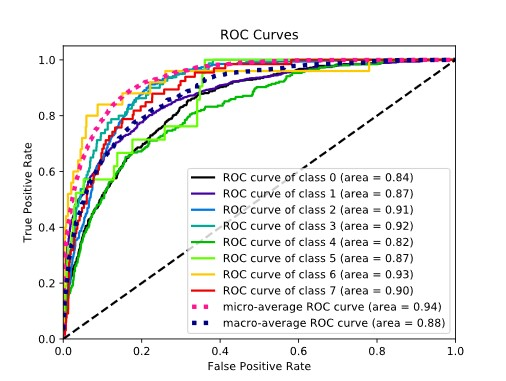
\includegraphics[width=1\linewidth]{pictures/SVM_ROC.jpg}  
	\caption{ROC Curves of the testing results}
	\label{SVM_ROC}
\end{figure}

\subsection{Consideration of Meta Data [TN]}
As already mentioned in the introduction there exsists additional data for most images called meta data. This contains information about the age, gender and the position of the skin lesion on the patients body. To make use of this additional data we convert each type into a one-hot vector and then attach all three vectors as additional input data. This improves the sensitivity score to 56.558\%.

